\subsection{Results}\label{ssec:M1:results}
In this section we present the results from our numerical simulations. Most of our results concern the evolution of various parameters as a function of $x$. Whenever it's relevant for interpreting and understanding the plot, we mark the point where we have matter-radiation equality and matter-dark energy equality, corresponding to $\om=\orad$ and $\om=\ol$, respectively. These points can be seen directly in \figref{fig:M1:results:omega_i_of_x}. 

\subsubsection{Analytical and numerical comparisons}
The dimensionless quantity $\eta\H/c$ is shown in \figref{fig:M1:results:compare_eta_H_over_c}. At the lowest values of $x\lesssim-10$, we see that $\eta\H/c=1$, as expected. Slightly before matter-radiation equality takes place, we see a slight increase towards higher $x$. As we approach higher $x$, $\ol$ starts dominating, and the solution eventually diverges, as expected.  
\begin{figure}[ht!]
    % 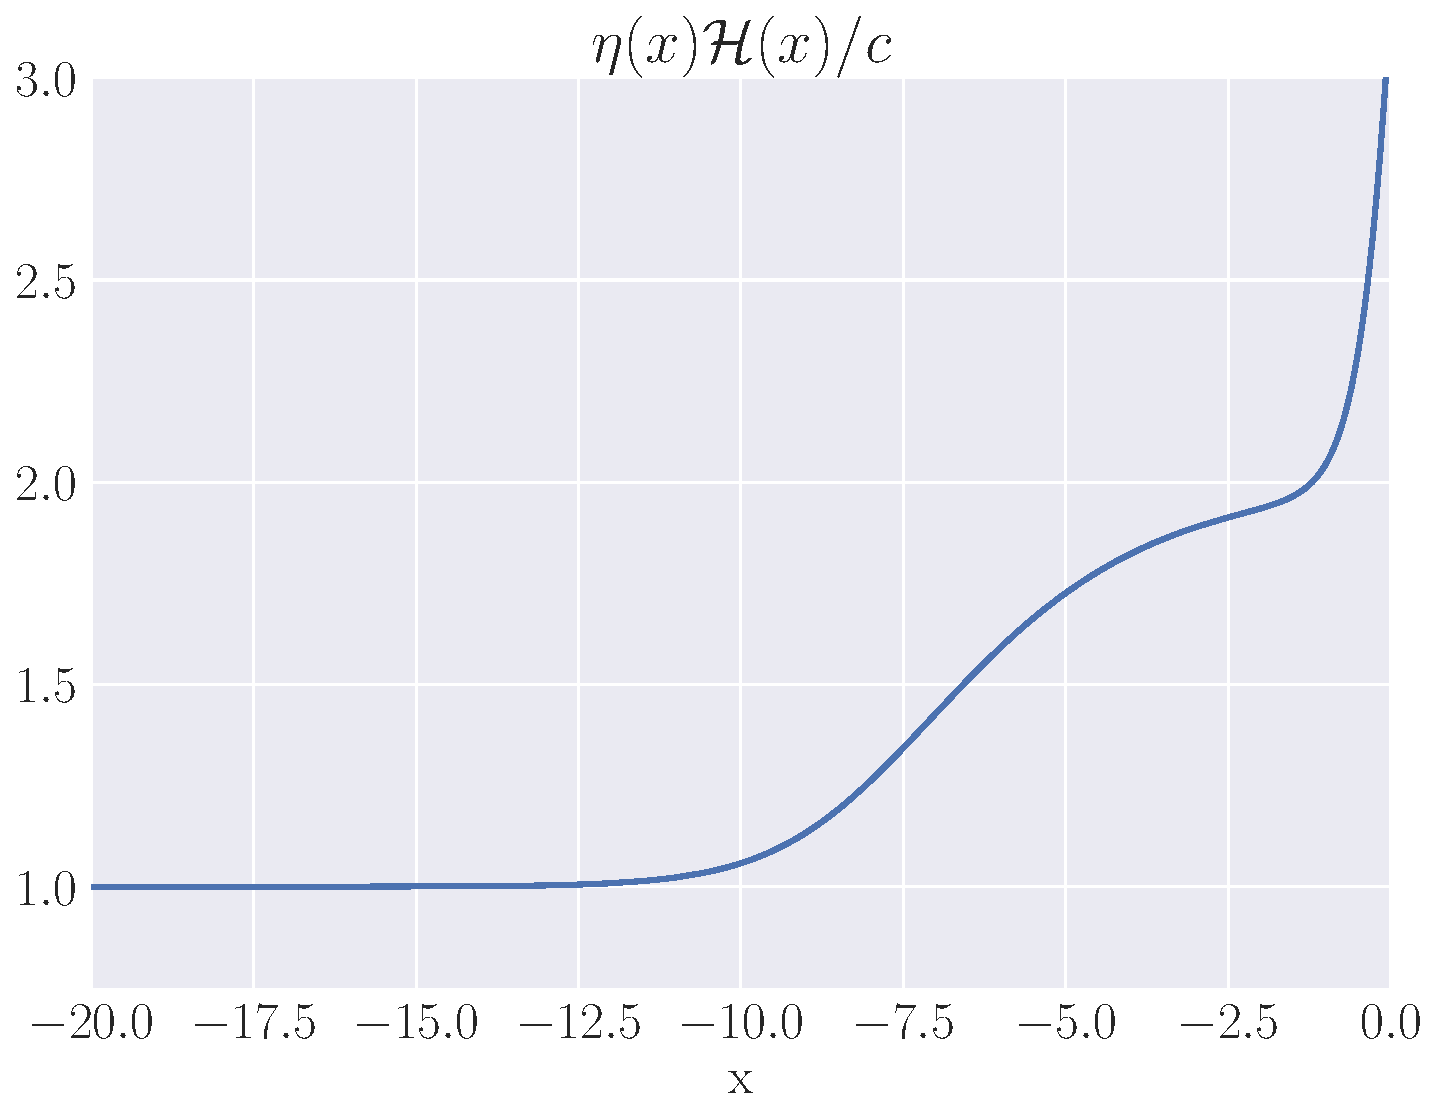
\includegraphics[width=\linewidth]{compare_eta_H_over_c.pdf}
    \includefig{compare_eta_H_over_c}
    \caption{The dimensionless quantity $\eta\H/c$ as a function of $x$. At low $x$ it has a value of $1$, as expected. The most significant changes occur near regions where there is a change in which density parameter is dominating.}
    \label{fig:M1:results:compare_eta_H_over_c}
\end{figure}

In \figref{fig:M1:results:dH_and_ddH_over_H} we have plotted $\H'/\H$ and $\H''/\H$, where we include the analytical approximation from \Eqref{eq:M1:theory:dH_dx_over_H_w} and \Eqref{eq:M1:theory:ddH_ddx_over_H_w}, respectively. The different values of $w$ are drawn over the whole range of $x$ where their related density parameter is larger than the other two. This is done for visibility purposes, and we only expect approximations to be reasonable whenever a density parameter is close to $1$. 

Towards the smallest values of $x$ we see that both quantities are well approximated by the analytical solutions for $w=1/3$. As we reach $x\gtrsim12$, matter becomes increasingly dominant, and the solution deviates from being purely dominated by a $w=1/3$ fluid. Towards the highest values of $x$, we see that both quantities reach a constant value of $1$ for $w=-1$. At higher values of $x$, we know that both $\om(x)$ and $\orad(x)$ should vanish, eventually, while $\ol\to1$. This behaviour is thus present in our implementation. When matter dominates, we see that both functions exhibit inferior agreement with the approximations compared to the other regimes. This can be understood from \figref{fig:M1:results:omega_i_of_x}, where the vanishing contribution of $\orad$ occurs around the same time as $\ol$ starts contributing. The maximum value reached for this particular configuration is $\om\approx0.995$. Nonetheless, significant deviations from the analytical solutions are not evident.
 
\begin{figure}[ht!]
    % 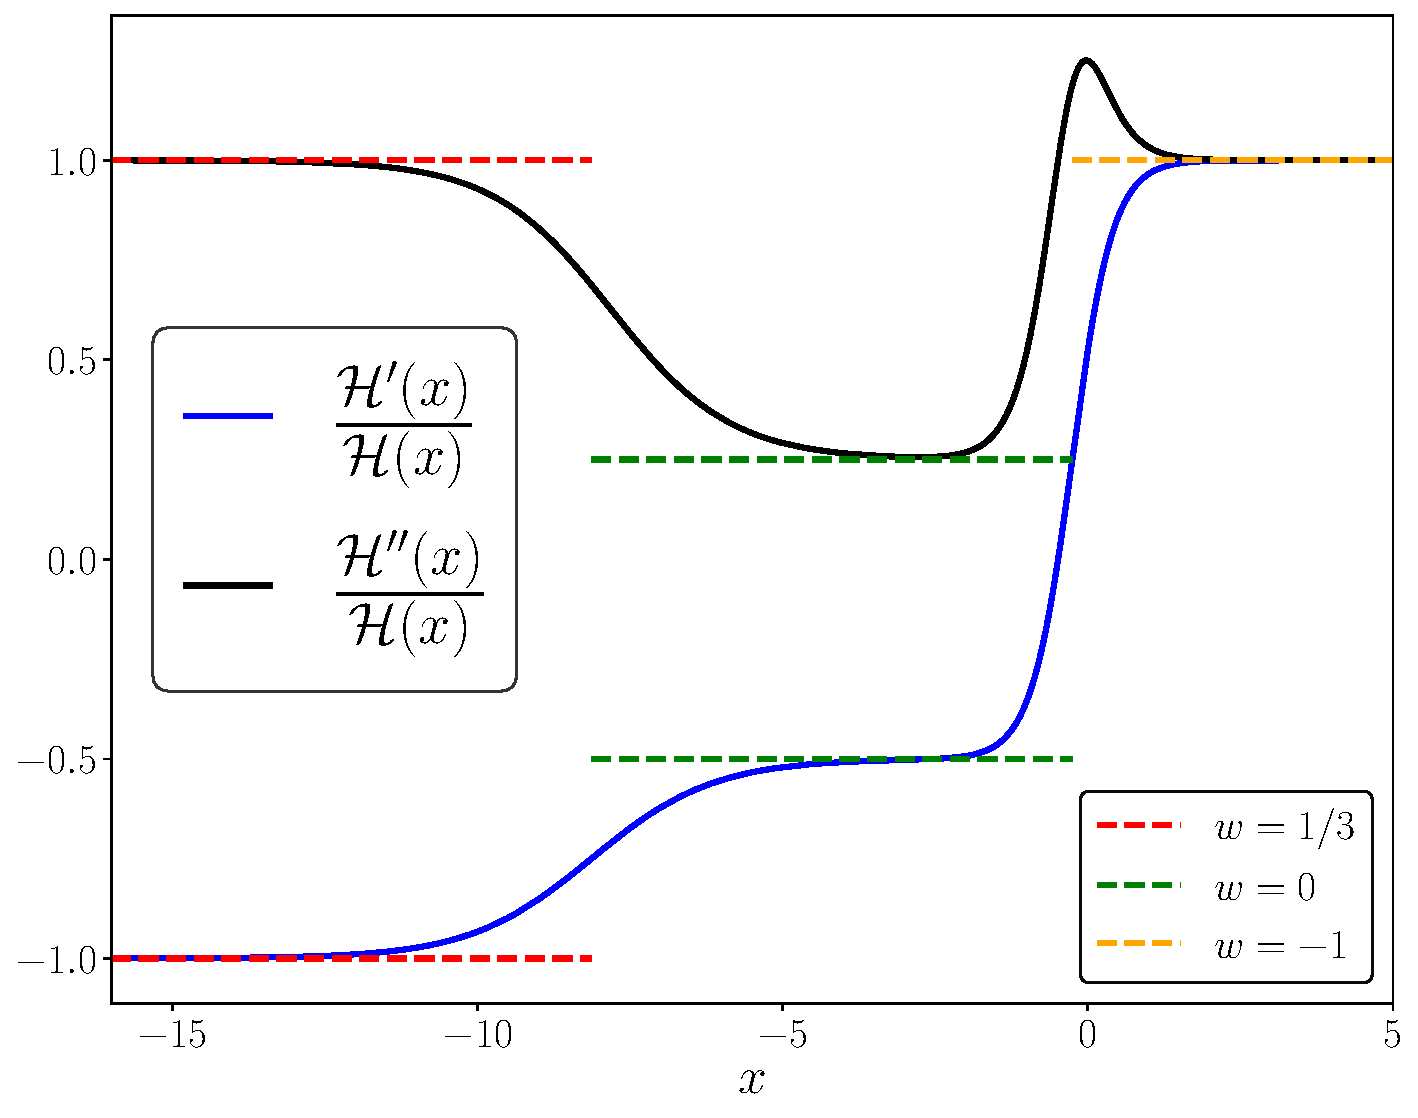
\includegraphics[width=\linewidth]{dH_and_ddH_over_H.pdf}
    \includefig{dH_and_ddH_over_H}
    \caption{$\H'/\H$ and $\H''/\H$ compared with analytical expressions in the case a single fluid with a given EoS parameter, $w$, shown by the dashed lines. The transition between the dashed lines are chosen as the corresponding epochs of equality.}
    \label{fig:M1:results:dH_and_ddH_over_H}
\end{figure}


\subsubsection{Hubble factor and time variables}
Having checked that our implementation is physical, we now proceed by studying the evolution of the background, starting with a plot of the conformal Hubble factor, $\Hx$, show in \figref{fig:M1:results:compare_Hp}.

The local minima taking place before matter-dark energy equality corresponds to the onset of acceleration, where $\ddot{a}=0$. For $x>0$, $\ol$ will dominate the conformal Hubble factor, where we have $\Hx\propto e^x$, as seen from \Eqref{eq:M1:theory:Hp_of_x}. 
\begin{figure}[ht!]
    % 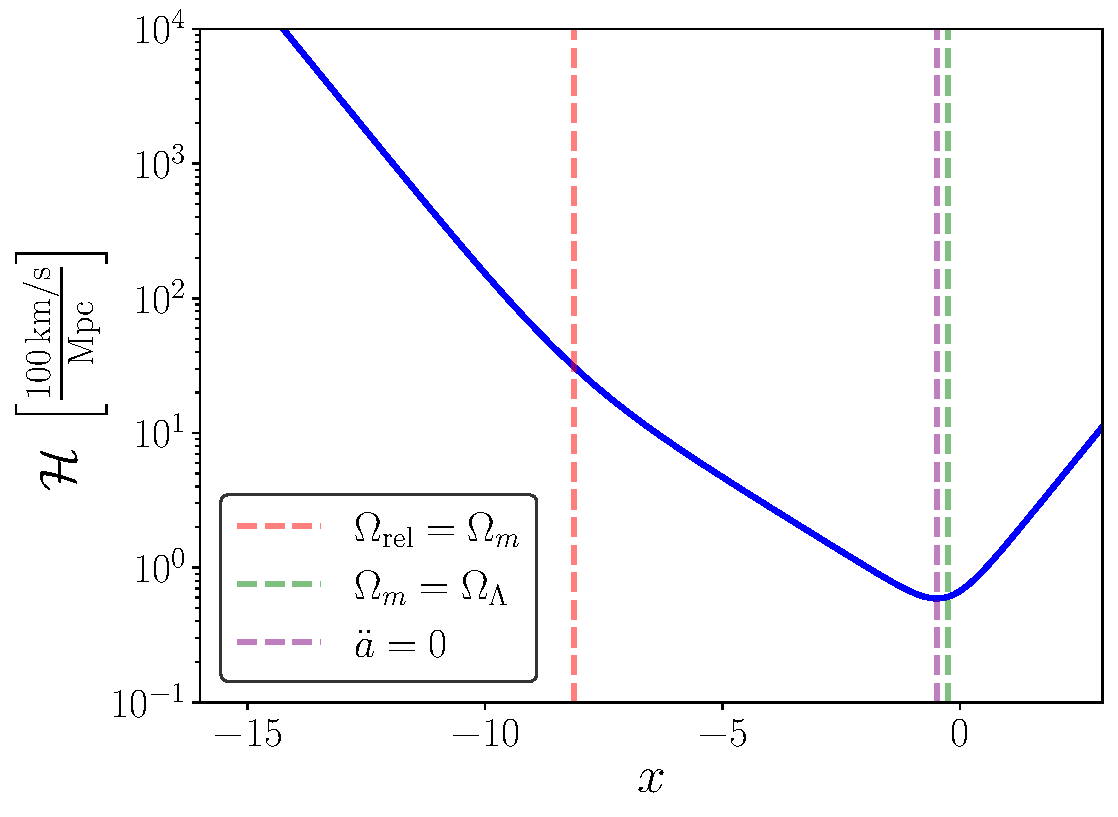
\includegraphics[width=\linewidth]{compare_Hp.pdf}
    \includefig{compare_Hp}
    \caption{Evolution of the conformal Hubble factor. The minimum point marks the onset of acceleration, after which, dark energy dominates its evolution.}
    \label{fig:M1:results:compare_Hp}
\end{figure}

The evolution of $\eta(x)$ and $t(x)$ is shown in \figref{fig:M1:results:t_and_eta_c}. At high values of $x$, the $e^x$ dependence of $\Hx$ causes $\eta(x)$ to grow as $e^{-x}$ at late times, suppressing its growth. The cosmic time, on the other hand, does not have an exponential dependence in the integrand at high values of $x$. This yields the linear growth we see at late times. The different $x$-dependece of $t$ and $\eta$ results in the two quantities to be approximately equal at $x\sim2.75$.    


\begin{figure}[ht!]
    % 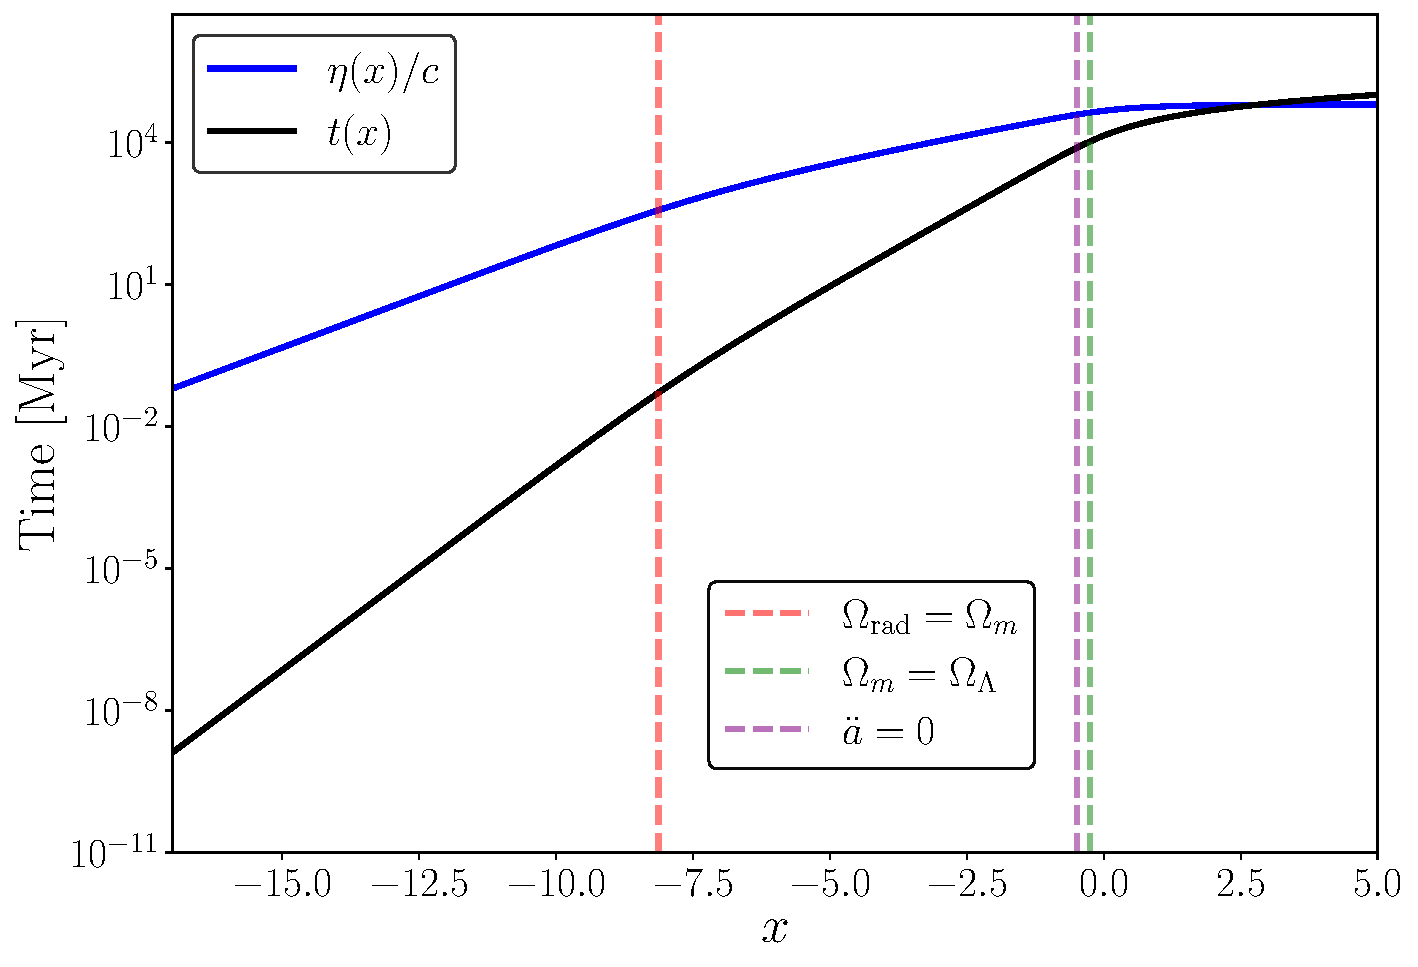
\includegraphics[width=\linewidth]{t_and_eta_c.pdf} 
    \includefig{t_and_eta_c}
    \caption{The cosmic time, $t$ and conformal time $\eta/c$. We emphasize that $\eta\neq t$ at small $x$, but the difference is discernable on the scale considered.}
    \label{fig:M1:results:t_and_eta_c}
\end{figure}


\begin{figure}[ht!]
    % 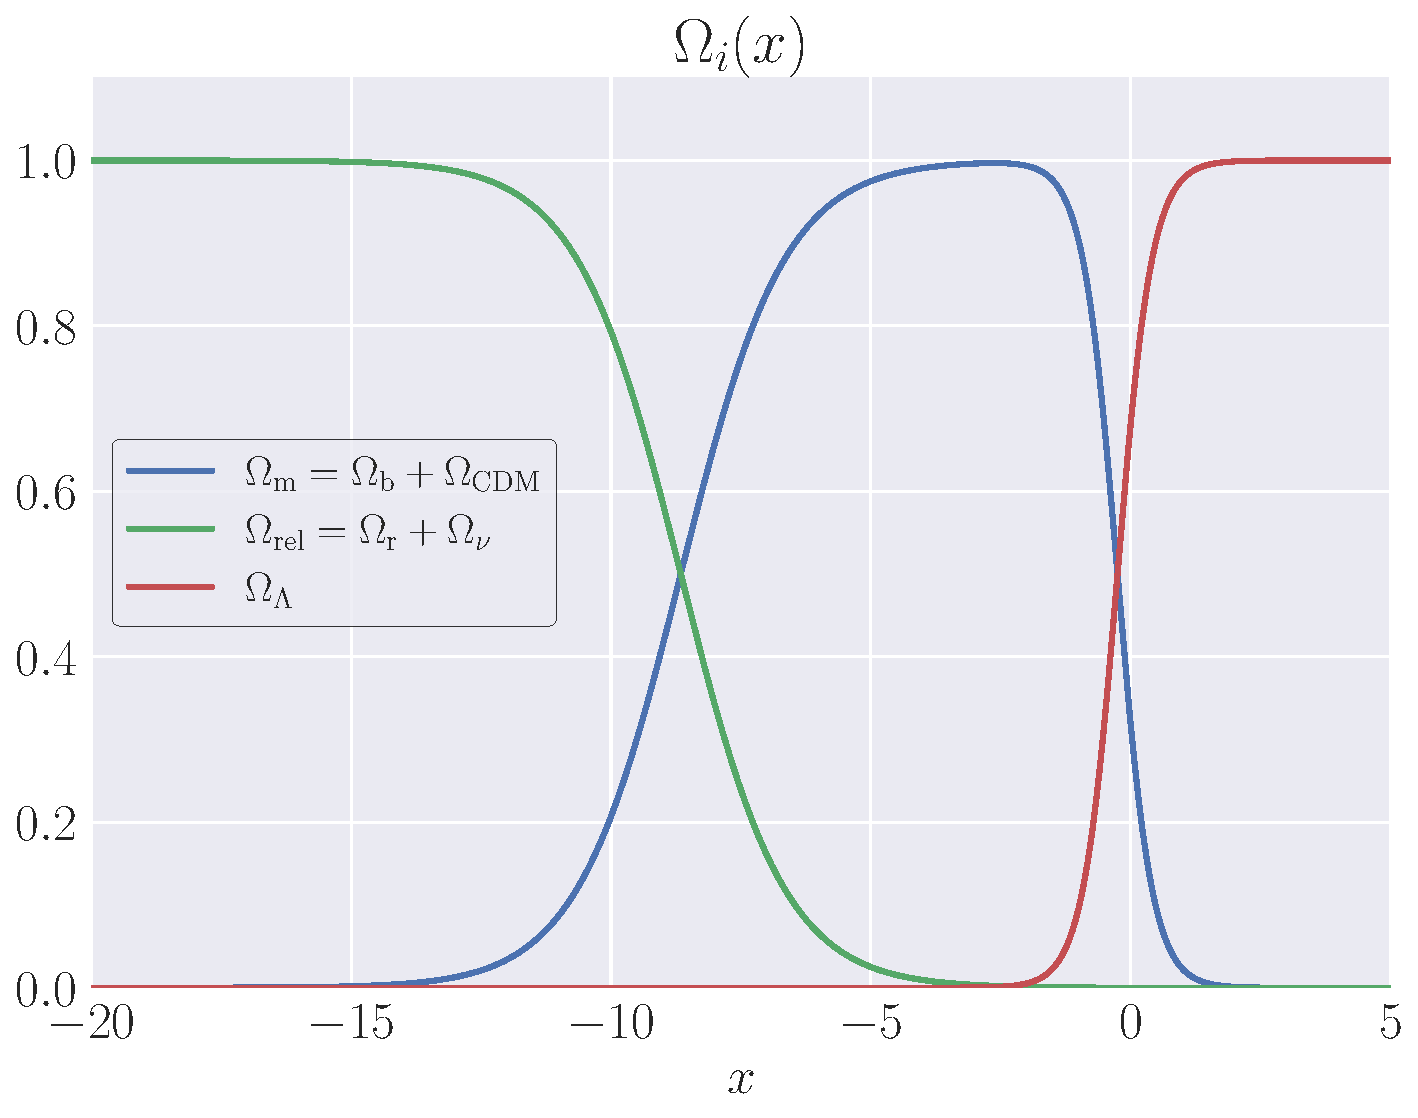
\includegraphics[width=\linewidth]{omega_i_of_x.pdf}
    \includefig{omega_i_of_x}
    \caption{Evolution of the density parameters over time. The points where $\om=\orad$ marks the epoch of matter-radiation equality, and the intersection between $\om$ and $\ol$ marks the epoch of matter-dark energy equality. The sum of the three quantities never exceed $1$, as expected.}
    \label{fig:M1:results:omega_i_of_x}
\end{figure}



\subsubsection{Supernova fitting}

A plot showing the luminosity distance as a function of redshift is shown in \figref{fig:M1:results:dL_z_compare_planck}, where we plot $d_L(z)/z$ to better compare the simulations with the data. There is a noticeable discrepancy between the simulated luminosity distance and the data, with most redshifts causing the simulation to fall outside the uncertainties.       
\begin{figure}[ht!]
    % 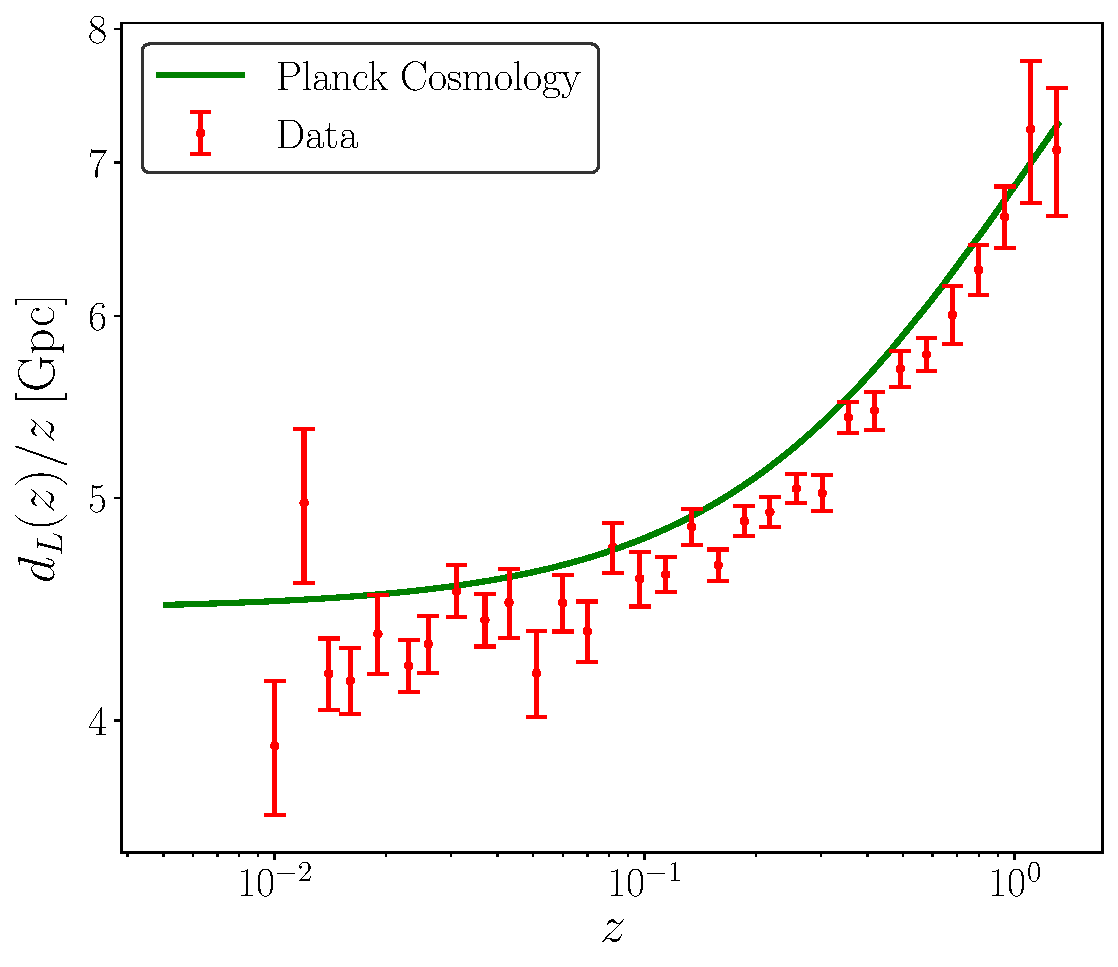
\includegraphics[width=\linewidth]{dL_z_compare_planck.pdf}
    \includefig{dL_z_compare_planck}
    \caption{Supernova data compared with the predicted luminosity distance obtained from simulations using Planck cosmology. Note that we use a logarithmic scale for the $y$-axis.}
    \label{fig:M1:results:dL_z_compare_planck}
\end{figure}

The $1\sigma$ and $2\sigma$ confidence regions in the $\ol-\om$ plane is shown in \figref{fig:M1:results:mcmc_supernova_fit_Nburn1000}. In the figure we have also indicated the parameter configuration for a flat Universe. A majority of the configurations seem to favour a non-flat Universe, with $\okn\approx 0.0674$. This could be a result of local variations in the gravitational field at small scales.      
\begin{figure}[ht!]
    % 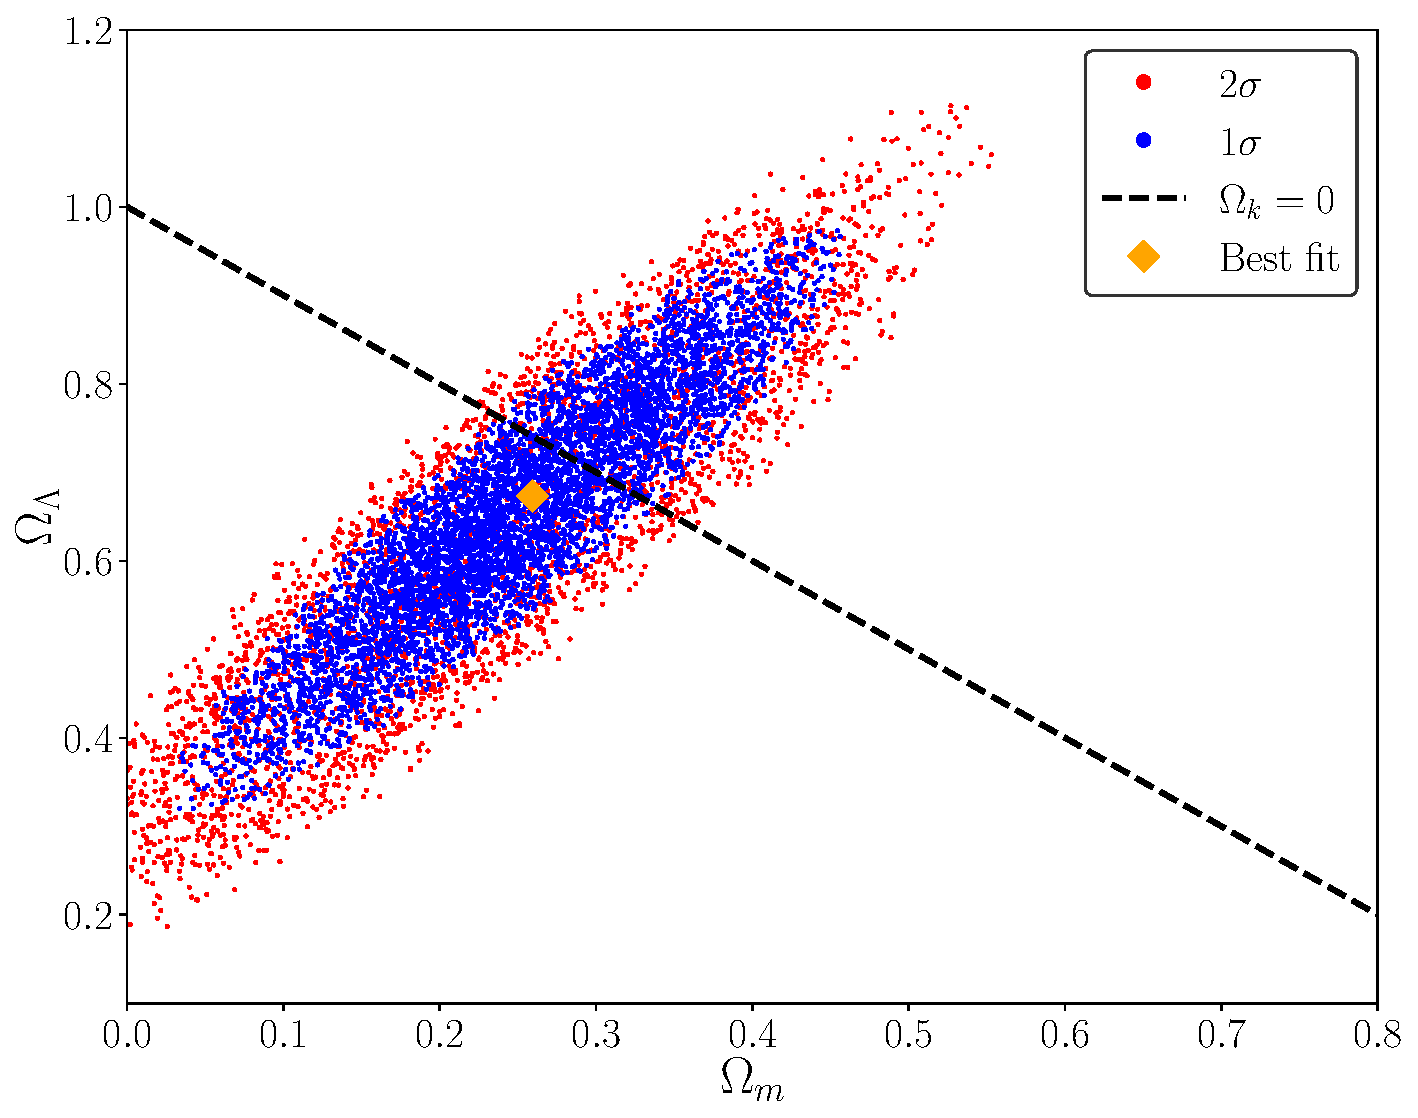
\includegraphics[width=\linewidth]{mcmc_supernova_fit_Nburn1000.pdf}
    \includefig{mcmc_supernova_fit_Nburn1000}
    \caption{Confidence regions of $\omn$ and $\oln$ obtained from fitting the supernova data. The best fit parameter values are shown in the plot, as well as the configurations that would give a flat Universe.}
    \label{fig:M1:results:mcmc_supernova_fit_Nburn1000}
\end{figure}

The posterior PDF of $H_0$ is shown in \figref{fig:M1:results:H0_pdf_Nburn1000}, where we have included the resulting Gaussian distribution from the mean and variance of the sampled $H_0$ values. This shows further discrepancy from the value of $H_0=67\unit{km/s/Mpc}$, given by Planck, while the mean value we obtain is $\hat{H}_0=70.1\unit{km/s/Mpc}$, with a corresponding standard deviation of $\hat{\sigma}_{H_0}=0.64\unit{km/s/Mpc}$.       
\begin{figure}[ht!]
    % 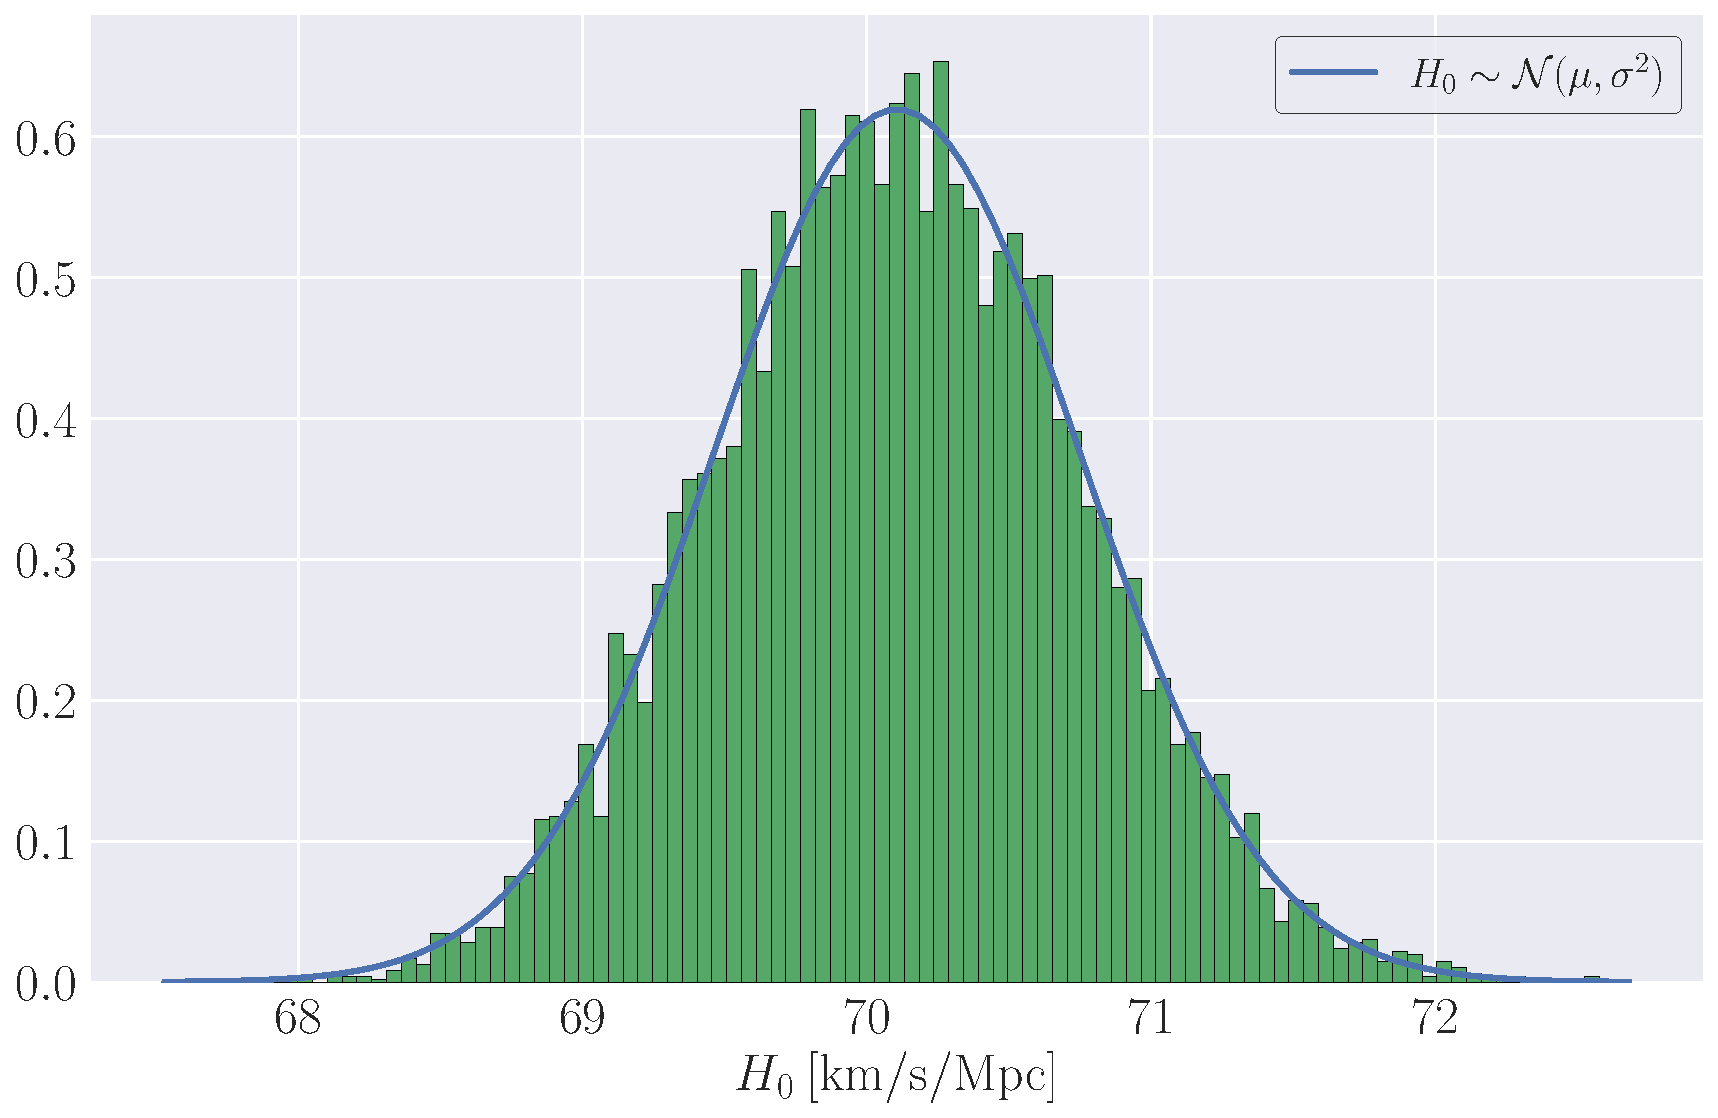
\includegraphics[width=\linewidth]{H0_pdf_Nburn1000.pdf}    
    \includefig{H0_pdf_Nburn1000}
    \caption{Posterior PDF of $H_0$. The histogram shows the sampled values, while the blue curve is the corresponding normal distribution obtained from the mean and variance of the data.}
    \label{fig:M1:results:H0_pdf_Nburn1000}
\end{figure}


With the fitted parameters, we can solve the background cosmology once again, and compute the resulting luminosity distance. The result is shown in \figref{fig:M1:results:dL_z_compare_fitted}, where the previous result from \figref{fig:M1:results:dL_z_compare_planck} is included for comparison purposes. The simulation with the best fit parameters yields a luminosity distance function that is much more consistent with data. However, there is still some discrepancy at lower redshift, but the associated data points in this regime have large uncertainties.    
\begin{figure}[ht!]
    % 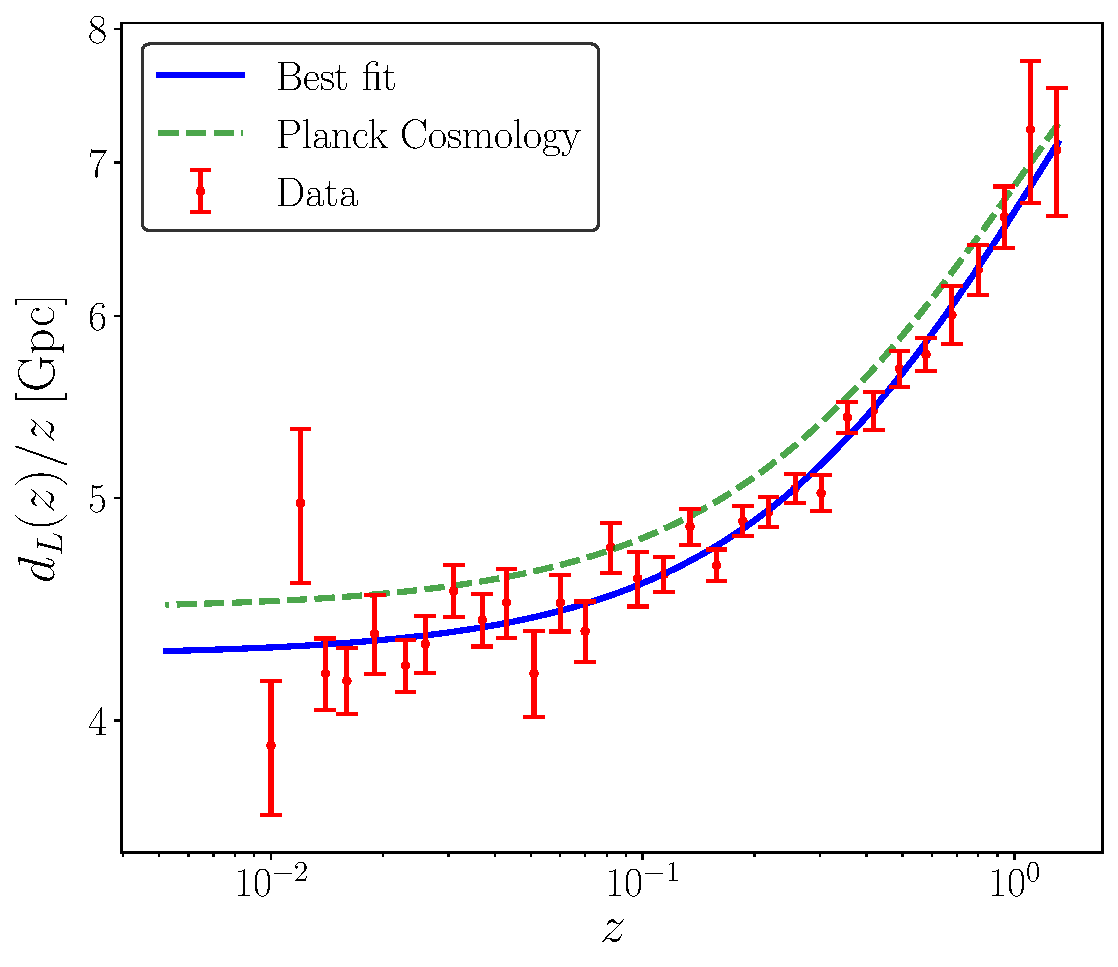
\includegraphics[width=\linewidth]{dL_z_compare_fitted.pdf}
    \includefig{dL_z_compare_fitted}
    \caption{The luminosity distance function obtained from the best fit values of $\C$ (blue line), compared with the result from the Planck cosmology (dashed green line), which is also shown in \figref{fig:M1:results:dL_z_compare_planck}.}
    \label{fig:M1:results:dL_z_compare_fitted}
\end{figure}


There are three important periods we have discussed, the times of matter-radiation equality, acceleration onset and matter-dark energy equality. The times when these incidents occur are listed in table \ref{tab:M1:results:time_values}, in terms of $x$, redshift $z$ and cosmic time $t$. We also include the age of the Universe today, $t_0\equiv t(x=0)$, and the conformal time today, $\eta_0/c$. 
\begin{table*}[ht!]
    \raggedright
    \begin{tabular}{l|ccccc}
\toprule
  & $\Omega_m=\Omega_r$ & $\Omega_m=\Omega_\Lambda$ & $\ddot{a}=0$ & $t_0$ & $\eta_0 / c$ \\
\midrule
$x$ & -8.13 & -0.26 & -0.49 & 13.85 & 46.29 \\
$z$ & 3400.32 & 0.29 & 0.63 & 13.85 & 46.29 \\
$t\unit{Gyr}$ & 51028.91$\unit{yr}$ & 10.37 & 7.75 & 13.85 & 46.29 \\
\bottomrule
\end{tabular}

    \label{tab:M1:results:time_values}
    \caption{Important times during the evolution of the Universe, expressed in terms of $x$, redshift and cosmic time. In the last two rows we also present today's time values}
\end{table*}